% Options for packages loaded elsewhere
\PassOptionsToPackage{unicode}{hyperref}
\PassOptionsToPackage{hyphens}{url}
%
\documentclass[
]{article}
\usepackage{lmodern}
\usepackage{amssymb,amsmath}
\usepackage{ifxetex,ifluatex}
\ifnum 0\ifxetex 1\fi\ifluatex 1\fi=0 % if pdftex
  \usepackage[T1]{fontenc}
  \usepackage[utf8]{inputenc}
  \usepackage{textcomp} % provide euro and other symbols
\else % if luatex or xetex
  \usepackage{unicode-math}
  \defaultfontfeatures{Scale=MatchLowercase}
  \defaultfontfeatures[\rmfamily]{Ligatures=TeX,Scale=1}
\fi
% Use upquote if available, for straight quotes in verbatim environments
\IfFileExists{upquote.sty}{\usepackage{upquote}}{}
\IfFileExists{microtype.sty}{% use microtype if available
  \usepackage[]{microtype}
  \UseMicrotypeSet[protrusion]{basicmath} % disable protrusion for tt fonts
}{}
\makeatletter
\@ifundefined{KOMAClassName}{% if non-KOMA class
  \IfFileExists{parskip.sty}{%
    \usepackage{parskip}
  }{% else
    \setlength{\parindent}{0pt}
    \setlength{\parskip}{6pt plus 2pt minus 1pt}}
}{% if KOMA class
  \KOMAoptions{parskip=half}}
\makeatother
\usepackage{xcolor}
\IfFileExists{xurl.sty}{\usepackage{xurl}}{} % add URL line breaks if available
\IfFileExists{bookmark.sty}{\usepackage{bookmark}}{\usepackage{hyperref}}
\hypersetup{
  hidelinks,
  pdfcreator={LaTeX via pandoc}}
\urlstyle{same} % disable monospaced font for URLs
\usepackage{graphicx,grffile}
\makeatletter
\def\maxwidth{\ifdim\Gin@nat@width>\linewidth\linewidth\else\Gin@nat@width\fi}
\def\maxheight{\ifdim\Gin@nat@height>\textheight\textheight\else\Gin@nat@height\fi}
\makeatother
% Scale images if necessary, so that they will not overflow the page
% margins by default, and it is still possible to overwrite the defaults
% using explicit options in \includegraphics[width, height, ...]{}
\setkeys{Gin}{width=\maxwidth,height=\maxheight,keepaspectratio}
% Set default figure placement to htbp
\makeatletter
\def\fps@figure{htbp}
\makeatother
\setlength{\emergencystretch}{3em} % prevent overfull lines
\providecommand{\tightlist}{%
  \setlength{\itemsep}{0pt}\setlength{\parskip}{0pt}}
\setcounter{secnumdepth}{-\maxdimen} % remove section numbering

\date{}

\begin{document}

\begin{enumerate}
\def\labelenumi{\arabic{enumi}.}
\setcounter{enumi}{2}
\tightlist
\item
  Abrir gerações
\end{enumerate}

Abrir geracoes junto com a matriz energetica

\hypertarget{introduuxe7uxe3o}{%
\section{Introdução}\label{introduuxe7uxe3o}}

Desde seus tempos mais remotos o homem busca soluções de facilitar sua
vida e seu esforço. seja por meio do uso de sistemas mecânicos ou até
mesmo recorrendo às forças de animais. Descoberta em meados do século
XVIII, por Benjamin Franklin\footnote{http://www.ifsc.usp.br/\textasciitilde cibelle/arquivos/T0150-1.pdf},
a eletricidade é sem sombra de dúvidas um grande avanço para a
incansável procura pela comodidade humana. Desde então a ciência está
sempre investigando formas de automatizar trabalhos complexos e
demorados com o uso de circuitos.

A geração de energia é um assunto muito pesquisado para os dias atuais.
Um motivo dessas pesquisas é o constante aumento de energia demandada,
seja para atividades domésticas ou serviços industriais. Para tais
problemas a eletrônica de potência tem grande colaboração na redução de
energia demandada, visando sempre o processamento eletrônico de energia,
causando maiores eficiências em circuitos, redução de volume e peso de
componentes, para que de tal forma a energia requerida pela população
seja menor.

Mesmo com a capacidade de geração de energia presente, em muitos lugares
a entrega de energia acaba sendo comprometida, seja pelas distâncias
entre subestações, ou até mesmo por eventuais faltas de sistemas
apropriados para uma eficiente distribuição. Em alguns casos até
mudanças climáticas acarretam em acidentes e imprevistos com o
fornecimento de energia, causando contratempos tanto para os
consumidores quanto para as próprias concessionárias.

Ao se fazer o projeto de uma usina, são feitos todos os levantamentos
referentes aos seus custos de instauração, licenciamento e
retorno.\footnote{https://www.hidroenergia.com.br/veja-quais-sao-as-etapas-para-construcao-de-uma-hidreletrica/}
Esses levantamentos ocasionalmente concluem que pode não ser possível
para a empresa a construção desse projeto, o que leva a um fornecimento
de energia debilitado até alguns clientes. Outro ponto refletido ao se
construir uma usina são os danos que provocados ao redor de sua
construção, danos os quais podem ser na parte ambiental, como o
desmatamento, a perfuração do solo, a inundação de lugares; ou até mesmo
sociais, como a isolação de terrenos para segurança da região ao redor
ou o ruído incômodo que será provocado. Esses pontos são também
problemas levados em consideração quando uma empresa quer construir uma
usina de grande porte.

Para tais problemas se faz importante o estudo completo de fontes de
geração e conversão de energia, seus custos, impactos e benefícios em
relação as outras formas. Do mesmo modo é necessário compreender as
naturezas de produção de energia e a matriz energética nacional e
mundial.

\hypertarget{matriz-energuxe9tica-atual}{%
\section{Matriz energética atual}\label{matriz-energuxe9tica-atual}}

A geração de energia no Brasil é em sua maior parte hidráulica, o que
não é ruim, pois a água é uma fonte renovável de energia, entretanto há
danos que são causados com a criação de usinas, como a inundação de uma
grande região, causando danos às pessoas que ficam desabrigadas, sem
contar à fauna e à flora. Entretanto, no mundo, a situação é outra: a
maior parte da energia mundial em cenário global é feita a base de
carvão mineral, uma matéria prima que não é renovável e difícil de ser
retirada do meio ambiente.

\hypertarget{sec:matriz_br}{%
\subsection{Brasil}\label{sec:matriz_br}}

Por mais que atualmente a maior parte da geração da energia elétrica
brasileira seja com base na água, é possível destacar um grande aumento
e incentivos(seja pelo governo ou pelos movimentos ambientais) de
gerações alternativas, como gás natural, biomassa e eólica. Este fato
pode ser observado na comparação dentre as figuras
{[}-@fig:brasil\_73{]} e {[}-@fig:brasil\_18{]} a seguir. Em 1999, a
maior parte da eletricidade provinha de hidrelétricas ao Brasil. Já em
2018, pôde-se notar uma grande mudança no cenário energético nacional.

\begin{figure}
\hypertarget{fig:brasil_73}{%
\centering
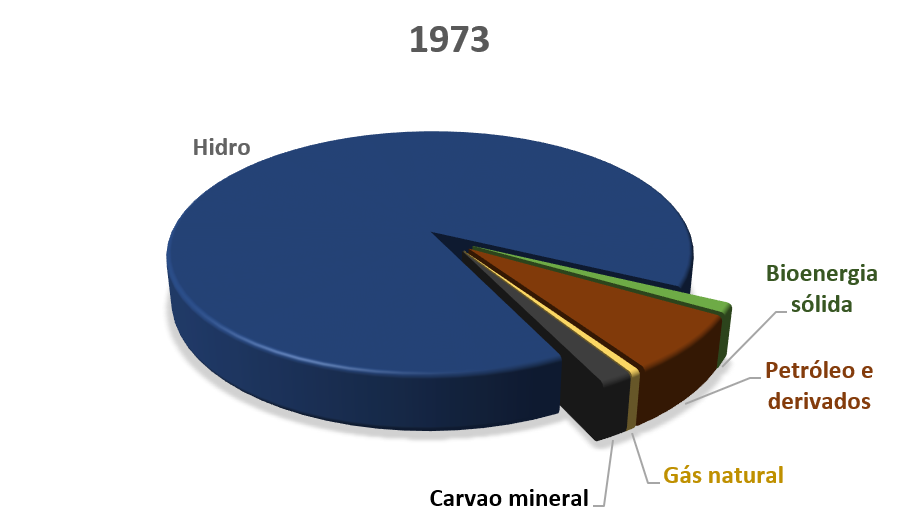
\includegraphics[width=3.125in,height=\textheight]{img/matriz/brasil_73.png}
\caption{Matriz elétrica brasileira - 1973, Fonte: MME, Autoria
própria}\label{fig:brasil_73}
}
\end{figure}

\begin{figure}
\hypertarget{fig:brasil_18}{%
\centering
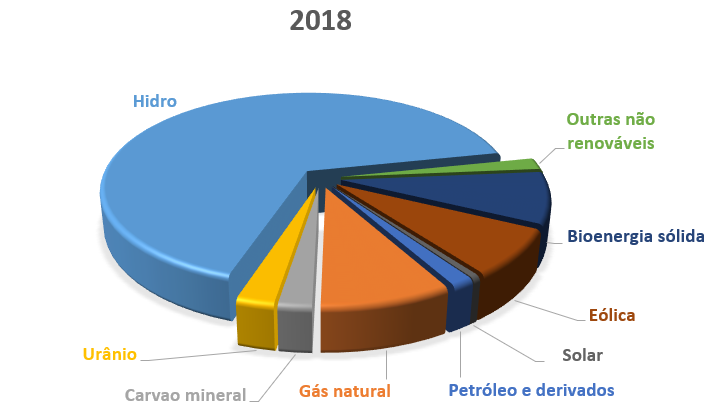
\includegraphics[width=3.125in,height=\textheight]{img/matriz/brasil_18.png}
\caption{Matriz elétrica brasileira - 2018, Fonte: MME, Autoria
própria}\label{fig:brasil_18}
}
\end{figure}

Também é perceptível o aumento da participação da geração de carvão
mineral, de 1.7\% a 2.2\%. Por mais que pareça ter aumentado em 0.5
pontos percentuais, na verdade a geração mineral brasileira serve para
cobrir faltas da geração hidráulica as quais não conseguem ser entregues
quando há períodos de secas, causadora do baixo nível nos reservatórios
das represas.\footnote{http://www.mme.gov.br/documents/1138787/1732840/Resenha+Energética+Brasileira+-+edição+2019+v2.pdf/66a837a8-4164-4b37-be4a-59a5ad270c50?version=1.0}

Outro fato importante a ser destacado é a diminuição percentual no uso
de hidrelétricas e Ascenção de outras fontes renováveis, tais como
eólica e bioenergia sólida. Com esse crescimento pode-se esperar também
a redução no uso da própria geração a base de carvão mineral.

\hypertarget{mundo}{%
\subsection{Mundo}\label{mundo}}

O cenário mundial apresenta as mesmas tendências, reduzindo o uso de
fontes não renováveis e das hidrelétricas, investindo também em fontes
renováveis capazes de entrega energia com menor custo em longo prazo. A
{[}@fig:mundo\_18{]} e a {[}@fig:mundo\_73{]} podem mostrar tal
comparação.

\begin{figure}
\hypertarget{fig:mundo_73}{%
\centering
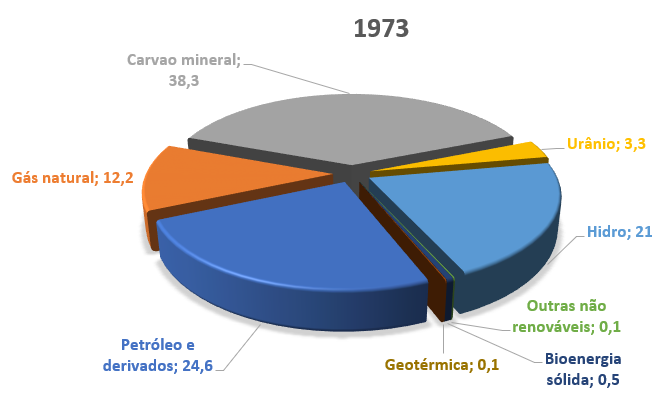
\includegraphics[width=3.125in,height=\textheight]{img/matriz/mundo_73.png}
\caption{Matriz elétrica mundial - 1973, Fonte: MME, Autoria
própria}\label{fig:mundo_73}
}
\end{figure}

\begin{figure}
\hypertarget{fig:mundo_18}{%
\centering
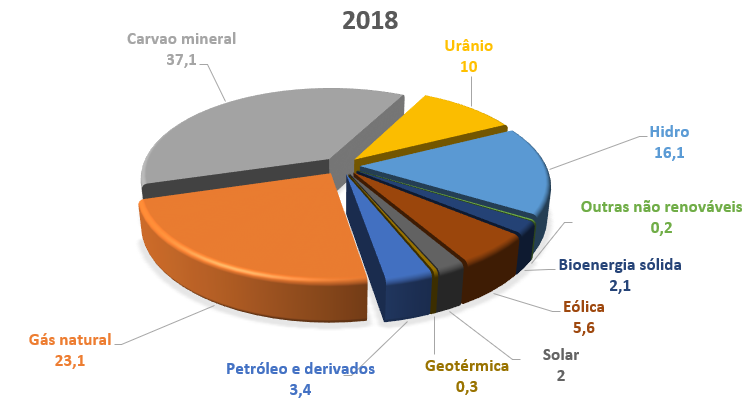
\includegraphics[width=3.125in,height=\textheight]{img/matriz/mundo_18.png}
\caption{Matriz elétrica mundial - 2018, Fonte: MME, Autoria
própria}\label{fig:mundo_18}
}
\end{figure}

A participação do petróleo para geração elétrica também diminuiu ao
redor do globo nos últimos 46 anos, revelando o interesse em fontes
inesgotáveis de energia.

\hypertarget{gerauxe7uxe3o-distribuida}{%
\section{Geração Distribuida}\label{gerauxe7uxe3o-distribuida}}

Nos últimos anos o mundo vem sofrendo mudanças climáticas e outros
desastres socioambientais decorrentes do desenfreado consumismo humano
do ultimo século. Estes desastres mostraram a todos que caso o planeta
não seja bem cuidado os dias do Homem podem estar contados. Tal fato tem
aumentado o receio de autoridades políticas. Com o crescimento desta
inquietação com o meio ambiente, muitas políticas estratégicas vêm sendo
elaboradas com o intuito da preservação do meio ambiente. Essas
políticas fazem parte da estratégia do desenvolvimento sustentável.

No Brasil estas políticas surgiram algum tempo depois, entretanto são
vistas como grandes propulsores para pessoas físicas e jurídicas, as
quais enxergam nestas políticas oportunidades de grandes negócios ou até
mesmo fontes para pequenos retornos e auxílios. Nos últimos vinte anos o
país tem elaborado planos de geração energética sustentável, com planos
de alavancar a nação para mais perto de outros países de
interesse\footnote{http://epe.gov.br/pt/publicacoes-dados-abertos/publicacoes/Plano-Nacional-de-Energia-PNE-2030}.
Redução em impostos e incentivos para produção de energia ``limpa'' como
à base de resíduos ou do vento são grandes exemplos destas políticas
nacionais.\footnote{https://www.camara.leg.br/noticias/561691-comissao-aprova-incentivo-a-geracao-de-energia-a-partir-de-residuos/}

Com tais incentivos, muitas pessoas acabam optado por instalar geradores
em suas residências. A geração própria implica na redução da demanda
energética do fornecedor. Isso faz com que a própria fatura de luz tenha
redução. O investimento em uma fonte de energia local tem também retorno
a longo prazo, devido a fatos como aumento da tarifa repassada pela
ANEEL.

Outrossim, há ocasiões pontuais em que o fornecimento de energia é
impossibilitado, seja por rompimento de cabos entre o consumidor e
distribuidor, interrupções programadas, acidentes no meio do trajeto do
fluxo da energia, ou até mesmo por maus projetos residenciais.\footnote{https://www.cpfl.com.br/energias-sustentaveis/eficiencia-energetica/uso-consciente/falta-de-energia/Paginas/default.aspx}
Como resolução de tais problemas a geração própria acaba sendo muito
favorável, possibilitando ao morador ou empresário o total funcionamento
de seu local de laboro.

Há momentos em que a tarifa de energia sofre alterações, as quais podem
ser ou não previstas. O que usualmente ocorre é o aumento de tarifa para
consumidores residenciais devido ao aumento de trabalho necessário para
fornecimento de eletricidade para as casas, o qual provém de níveis
baixos nos reservatórios das usinas. Como já comentado na
{[}@sec:matriz\_br{]}, como a maior parte da energia depende do setor
hidráulico, em períodos de seca são necessárias mais usinas
trabalhando.\footnote{http://www.aneel.gov.br/bandeiras-tarifarias}
Esses valores de tarifas possuem o nome de ``bandeiras tarifárias''. Um
outro ``aumento'' de tarifa pode ser notado em indústrias, no que
comumente é chamado de ``horário de ponta'', definido como um período de
três horas consecutivas, as quais há um grande acréscimo de energia
demandada para a empresa concessionária, a qual, preservada por leis,
cobra a energia consumida nessa faixa a uma tarifa específica,
logicamente com seu valor mais elevado.\footnote{http://www.mme.gov.br/documents/10584/1985241/Manual\%20de\%20Tarif\%20En\%20El\%20-\%20Procel\_EPP\%20-\%20Agosto-2011.pdf}

Com a produção de energia particular, entretanto, o consumo no período
de ponta pode ser totalmente com base na mesma energia produzida,
fazendo com que o consumo tarifado seja nulo. De mesmo modo, nos
períodos de bandeiras tarifárias vermelhas e amarela, o consumo a ser
pago encaminha-se ao consumo mínimo, o qual é obrigatório ser
pago.\footnote{http://www2.aneel.gov.br/arquivos/PDF/Cartilha\_1p\_atual.pdf}

Não obstante, a geração particular de energia acarreta em uma menor
demanda para a companhia elétrica responsável pela região, o que também
diminui a demanda energética das usinas geradoras de maiores portes. O
que essa diminuição da demanda implica é a dispensabilidade de projetos
para construção de novas usinas. Esses projetos que, como já discutido,
trazem consigo vários percalços.

A partir de 17 de abril de 2012, qualquer consumidor brasileiro pode
produzir sua própria energia, desde que oriunda de fontes renováveis ou
por ``cogeração qualificada''.\footnote{http://www2.aneel.gov.br/cedoc/ren2012482.pdf}
Já em lugares de maior porte, como indústrias e hospitais, pode-se fazer
uso também de geradores a combustão de derivados do petróleo, seja
apenas em horário de ponta ou quando há comprometimento na entrega de
energia. Faz-se importante então um estudo a respeito dessas fontes de
energia.

\hypertarget{gerauxe7uxe3o-a-combustuxe3o}{%
\subsection{Geração a combustão}\label{gerauxe7uxe3o-a-combustuxe3o}}

Os geradores a diesel ou gasolina estão presentes na maioria das
indústrias e hospitais, tanto para atender às necessidades em momentos
que ocorre falta de energia, ou até para uso no período de ponta, com o
intuito de reduzir as contas.

O funcionamento do gerador a combustão baseia-se na lei de Faraday
({[}@eq:leifaraday{]}), onde a variação de campo magnético conduz na
produção de um campo elétrico, também variável. O combustível causa
explosões nos pistões do gerador, os quais são responsáveis para dar
movimento ao rotor.

\[ \oint \vec{E} \cdot d\vec{s} = -\frac{d\phi_B}{dt} \]\{\#eq:leifaraday\}

Essas máquinas contemplam o gerador propriamente dito acoplado com um
motor, o qual é impulsionado a partir de fluidos, como diesel, óleos
pesados, GLP, ou outros derivados do petróleo. Toda a rotação é gerada a
partir da explosão desses fluidos nos pistões do motor (figuras
{[}-@fig:diesel1{]} e {[}-@fig:diesel2{]}).

\begin{figure}
\hypertarget{fig:diesel1}{%
\centering
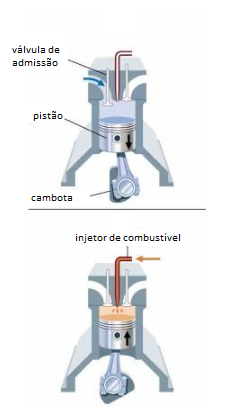
\includegraphics[width=\textwidth,height=3.125in]{img/gerador/motor1.png}
\caption{Admissão (A) e Compressão (B) do ar em motores de
combustão}\label{fig:diesel1}
}
\end{figure}

\begin{figure}
\hypertarget{fig:diesel2}{%
\centering
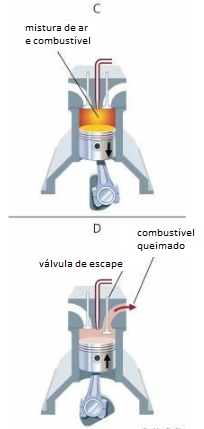
\includegraphics[width=\textwidth,height=3.125in]{img/gerador/motor2.png}
\caption{Expansão (A) e Escape (B) dos gases da combustão motores de
combustão}\label{fig:diesel2}
}
\end{figure}

Em geradores de campo giratório, como o da {[}@fig:rotorgiratório{]}, a
tensão é extraída diretamente dos enrolamentos da armadura
(estator).\footnote{https://static.weg.net/medias/downloadcenter/h68/h68/WEG-curso-dt5-caracter-sticas-e-especifica-o-de-geradores-artigo-tecnico-portugues.pdf}
Com a movimentação do motor, um campo elétrico é induzido na armadura,
donde flui corrente elétrica.

\begin{figure}
\hypertarget{fig:rotorgiratuxf3rio}{%
\centering
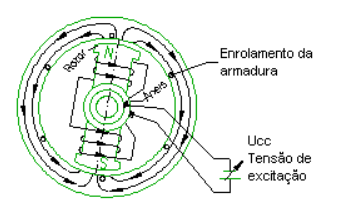
\includegraphics[width=2.08333in,height=\textheight]{img/gerador/geradorarmadurafixa.png}
\caption{Esquema de gerador elemental com armadura fixa -
Fonte:WEG}\label{fig:rotorgiratuxf3rio}
}
\end{figure}

O formato da onda de saída depende do formato que o campo possui em
relação ao tempo, os geradores são construídos com a finalidade de
produzir ondas em formato senoidal.

Como a geração a combustão produz gás carbônico como resultado, a lei
permite o uso dessas máquinas em pequenas faixas ao longo do dia,
objetivando uma menor poluição por parte das empresas.

\hypertarget{gerauxe7uxe3o-euxf3lica}{%
\subsection{Geração eólica}\label{gerauxe7uxe3o-euxf3lica}}

Assim como geradores a combustão, a geração eólica toma como base o
princípio da conversão de energia mecânica em elétrica por meio da lei
de Faraday, a qual testifica a presença de uma força eletromotriz
induzida resultante de uma variação de campo magnético sentido pelo
circuito.\footnote{http://www.ifsc.usp.br/\textasciitilde strontium/Teaching/Material2010-2\%20FFI0106\%20LabFisicaIII/11-LeideInducaodeFaraday.pdf}

A rotação da turbina dos aerogeradores se dá a partir do movimento do
vento, que é captado pelas pás. Devido ao tamanho que as pás captadoras
possuem, sua rotação não atinge os valores necessários para conversões
diretas, então é crucial o uso de caixas de engrenagens, designadas a
multiplicar a velocidade de rotação a ser acoplada ao seu respectivo
gerador ({[}@fig:componentes\_turbina{]}).

\begin{figure}
\hypertarget{fig:componentes_turbina}{%
\centering
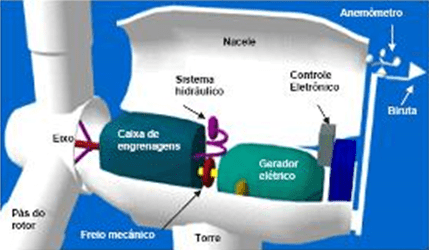
\includegraphics[width=3.125in,height=\textheight]{img/eolico/componente-da-turbina.png}
\caption{Componentes de uma turbina
eólica}\label{fig:componentes_turbina}
}
\end{figure}

O anemômetro é capaz de aferir a intensidade, velocidade e direção do
vento, dando possibilidade de controlar a angulação das pás, para melhor
aproveitamento tanto de rotação quanto da geração.

Mesmo sendo uma fonte de energia renovável e não poluente, a geração
eólica ainda traz consigo algumas adversidades. O ar, ao se chocar com
as pás, provoca ruídos desconfortáveis para a população próxima. Outro
problema a ser citado é o impacto que animais voadores podem causar nas
pás, trazendo danos para a produção e diminuindo a vida útil dos
equipamentos.

Outro ponto observado é a intermitência que os ventos possuem, sendo
provável que em certos momentos de maior demanda não haja vento soprando
suficiente, ou até mesmo em situações de demanda em que não há vento
algum, trazendo para a geração eólica uma inconstância indesejada.

\hypertarget{gerauxe7uxe3o-fotovoltaica}{%
\subsection{Geração fotovoltaica}\label{gerauxe7uxe3o-fotovoltaica}}

Dentre os atuais meios de se produzir energia elétrica, um que está
sempre em voga é a geração fotovoltaica. Essa geração é silenciosa e
abundante. Outro fator que contribui para a geração de energia através
do sol é que a estrela tem uma vida muito longa, e inesgotável,
comparada ao tempo humano na terra. A energia irradiada na Terra chega a
\(9,5.10^4\) terawatts, até 10 mil vezes toda a energia consumida no
planeta\footnote{Grätzel, M. Photoelectrochemical cells. Nature 2001,
  414, 338. {[}CrossRef{]}}.

As células, em trabalho, não produzem gases ou efluentes, fazendo assim
com que o meio ambiente não seja afetado na produção de energia. Este
fator é também outro motivo que aponta a vantagem da energia solar em
relação às outras formas de geração, e um assunto que é discutido
hodiernamente devido à conscientização ambiental a qual muito se fala
atualmente.

\hypertarget{efeito-fotovoltaico}{%
\subsubsection{Efeito fotovoltaico}\label{efeito-fotovoltaico}}

Atualmente, muito se comenta a respeito da energia solar e sua geração
com os painéis e módulos fotovoltaicos. Há muitas pesquisas nesse meio,
com objetivos como tornar a tecnologia mais próxima do público. A
unidade mais simples para a formação dos módulos são as células.

A célula fotovoltaica tem seu funcionamento oriundo do efeito
fotovoltaico. Este fenômeno é mais antigo do que a maioria das pessoas
pensam. Em 1839, Edmond Becquerel percebeu a geração de energia a partir
de luz solar incidindo em placas de latão submersas em um líquido
eletrólito \footnote{Smestad, G. P. Optoelectronics of solar cells, 1a.
  ed., SPIE: Bellingham, 2002.}. Mais tarde, então, Charles Frittts foi
capaz de inventar a primeira bateria de luz solar, feita com base em
selênio\footnote{Komp, R. J. Practical photovoltaics: eletricity from
  solar cells, 3a. ed., aatec publications: Ann Arbor, 2001.}.

Atualmente as células são fabricadas com semicondutores, materiais que
apresentam características intermediárias entre condutores e isolantes.
O elemento mais famoso dentre os semicondutores é o silício. O cristal
de silício puro é mal condutor elétrico, devido ao fato de conter 4
elétrons livres em sua camada de valência. Para que a condução seja
possível, acrescentam-se porcentagens de outros elementos, com a
finalidade de deixar o átomo quase estável. A este processo dá-se o nome
de ``dopagem''.

A partir da dopagem do silício com o arsênio ou o fósforo, elementos que
apresentam 5 elétrons na última camada, formam-se ligações covalentes
entre quatro elétrons, o quinto é propositalmente livre, possibilitando
a passagem de corrente elétrica. Por ser dopado com elétrons a mais, é
nomeado silício tipo N.

A dopagem do silício tipo P é geralmente feita à base de gálio ou boro,
elementos com três elétrons na camada mais distante. Agora são feitas
três ligações covalentes, a quarta ligação é propositalmente ausente, e
também chamada de lacuna({[}@fig:dopagem{]}).

\begin{figure}
\hypertarget{fig:dopagem}{%
\centering
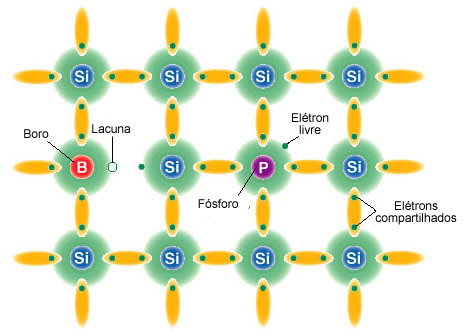
\includegraphics[width=3.125in,height=\textheight]{img/fotovoltaico/dopagem_eletronica.jpg}
\caption{Dopagem Eletrônica, Fonte: Infoescola}\label{fig:dopagem}
}
\end{figure}

A célula fotovoltaica contem as duas dopagens, sendo uma camada fina de
material tipo N e uma camada espessa de material do tipo P, conforme
ilustra a {[}@fig:transversal{]}. Com isso, é gerado um campo elétrico,
também chamado de região PN\footnote{https://www.solenerg.com.br/files/monografia\_cassio.pdf}.
Quando a luz incide na célula, os elétrons recebem energia proveniente
dos fótons. Os elétrons, então excitados, são acelerados e fluem através
da junção. A corrente gerada origina a diferença de potencial entre as
faces P e N.\footnote{https://www.solenerg.com.br/files/monografia\_cassio.pdf}

\begin{figure}
\hypertarget{fig:transversal}{%
\centering
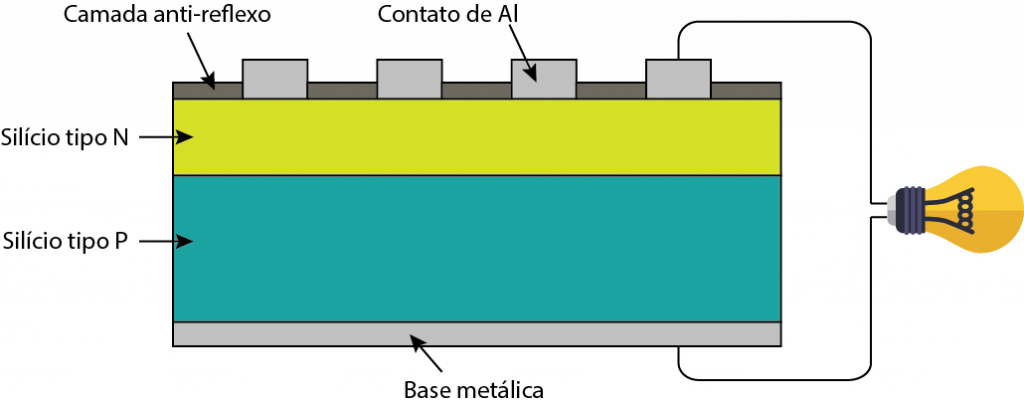
\includegraphics[width=3.125in,height=\textheight]{img/fotovoltaico/placatransversal.png}
\caption{Visão lateral de uma célula
fotovoltaica}\label{fig:transversal}
}
\end{figure}

\hypertarget{cuxe9lulas-fotovoltaicas}{%
\subsubsection{Células fotovoltaicas}\label{cuxe9lulas-fotovoltaicas}}

\textbf{falar dos tipos de paineis monocristalino e policristalino}

\hypertarget{referuxeancias}{%
\section{Referências}\label{referuxeancias}}

\end{document}
